\documentclass[10pt]{beamer}
% \documentclass[handout,10pt]{beamer}
\usepackage{my_style}

\title[Math/CS 375]{Lecture 09 - A}
\subtitle{\S 4.1 Polynomial Interpolation }

\begin{document}
% -------------------------------------------------
\begin{frame}
  \titlepage
\end{frame}
% -------------------------------------------------

\begin{frame}{Goals}
We will answer these questions:\\[3mm]
\begin{itemize}
    \item What is numerical interpolation supposed to accomplish?
    \item What is a monomial basis and what are its drawbacks?
    \item What is the Lagrange basis and why is it better?
    \item What is the Newton basis and why is it better than both the monomial and Lagrange?
\end{itemize}
\end{frame}

%%%%%%%%%%%%%%%%%%%%%%%%%%%%%%%%%%%%%%%%%%%%%%%%%%%%%%%%%%%%%%%%%%%%%%%%%%%%%%%%%%%%%%
\begin{frame}{Math Joke}

What is the next number in the sequence? 
$$ 1, 2, 3,\underline{\hspace{ 6 mm}} $$

\onslide<2->{
It's $\pi$! Plug in 1, 2, 3, and then 4 into the polynomial 
$$ p(x) = \frac{\pi x^3}{6} - \frac{2 x^3}{3} - \pi x^2 + 4 x^2 + \frac{11 \pi x}{6} - \frac{19 x}{3} - \pi + 4 $$


\begin{center}
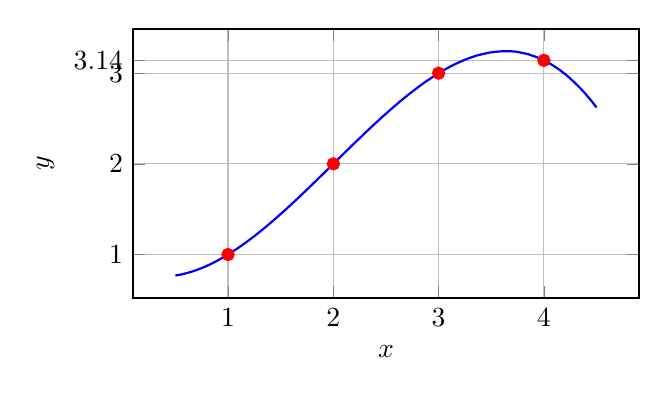
\begin{tikzpicture}
    \begin{axis}[
        width=8cm, height=5cm,
        xlabel={$x$}, ylabel={$y$},
        grid=major, 
        thick,
        domain=0.5:4.5, % Limiting the domain to show relevant points
        samples=100,
        xtick={1,2,3,4},
        ytick={1,2,3,3.14},
        legend pos=outer north east
    ]
    % Polynomial curve
    \addplot[color=blue, thick] {(pi*x^3)/6 - (2*x^3)/3 - pi*x^2 + 4*x^2 + (11*pi*x)/6 - (19*x)/3 - pi + 4};

    % Points at x=1, 2, 3, 4
    \addplot[color=red, only marks, mark=*] 
        coordinates {(1,1) (2,2) (3,3) (4,3.1416)};

    \end{axis}
\end{tikzpicture}
\end{center}
}
\end{frame}



%%%%%%%%%%%%%%%%%%%%%%%%%%%%%%%%%%%%%%%%%%%
\sectionframe{Data Points}
%%%%%%%%%%%%%%%%%%%%%%%%%%%%%%%%%%%%%%%%%%%
\begin{frame}{Working with Data Points}
  \begin{block}{Objective}
  Given a set of data points, find an approximating function $g(x)$ to represent the data.  
  \end{block}
\vspace{5mm}
Why?\\
\begin{itemize}
    \item Data analysis 
    \item Prediction 
    \item Scientific modeling 
\end{itemize}
\vspace{5mm}
Types of approximating functions:
\begin{enumerate}
  \item Polynomials
  \item Piecewise polynomials
  \item Rational functions
  \item Trig functions
\end{enumerate}
\end{frame}
%%%%%%%%%%%%%%%%%%%%%%%%%%%%%%%%%%%%%%%%%%%
\begin{frame}{Curve Fitting}


\begin{itemize}
    \item  The goal of \textbf{Curve fitting} is to find a continuous function that represents discrete data.

    \item Interpolation and Regression are forms of curve fitting
    
\end{itemize}
\vfill
\begin{block}{Interpolation}
    Construct a function $f(x)$ that cuts through all data points. 
\end{block}
\vfill 
\begin{block}{Regression}
    Find parameters for a function $f_p(x)$ that has a low over-all error at data points.
\end{block}
\vfill

\end{frame}
%%%%%%%%%%%%%%%%%%%%%%%%%%%%%%%%%%%%%%%%%%%
\begin{frame}{Interpolation}
\begin{center}
    
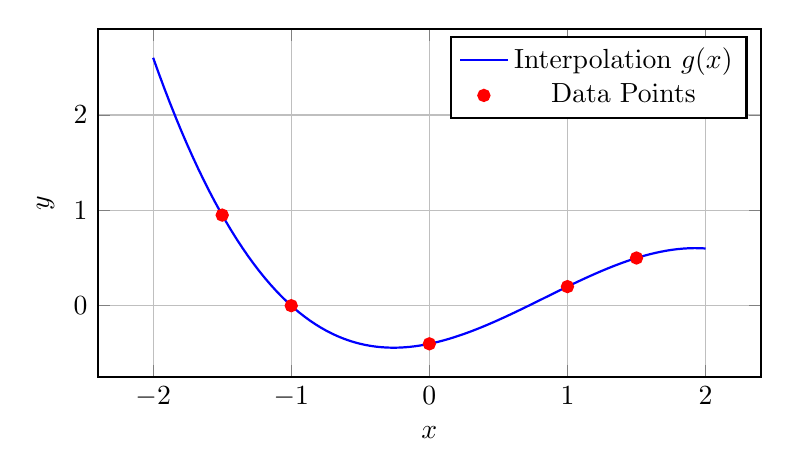
\begin{tikzpicture}
    \begin{axis}[
        width=10cm, height=6cm,
        xlabel={$x$}, ylabel={$y$},
        grid=major, 
        thick,
        domain=-2:2,
        samples=100,
        % legend pos=outer south
    ]
    % Polynomial interpolation curve
    \addplot[color=blue, thick] {-0.2*x^3 + 0.5*x^2 + 0.3*x - 0.4};

    % Interpolation points
    \addplot[color=red, only marks, mark=*] 
        coordinates {(-1.5,0.95) (-1, 0) (0, -0.4) (1, 0.2) (1.5, 0.5)};
    
    % Optional legend
    \legend{Interpolation $g(x)$, Data Points};
    \end{axis}
\end{tikzpicture}\\
\textbf{Interpolation}: function cuts through all data points
\end{center}
\end{frame}


\begin{frame}{Regression}
\begin{center}
    
    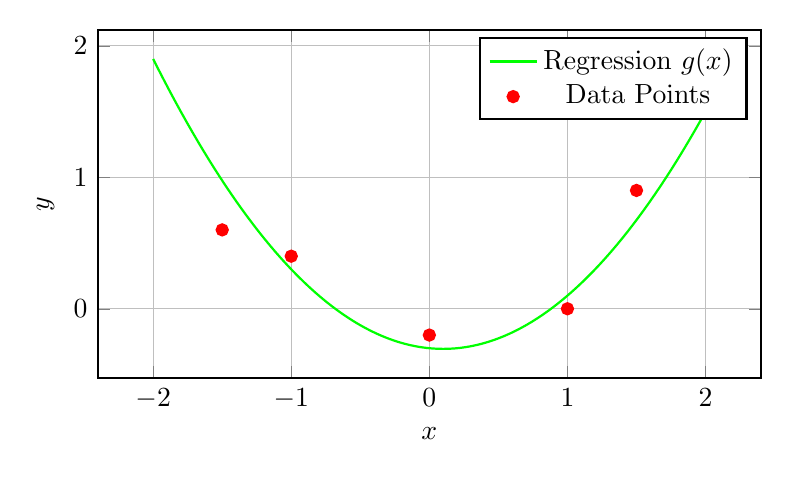
\begin{tikzpicture}
    \begin{axis}[
        width=10cm, height=6cm,
        xlabel={$x$}, ylabel={$y$},
        grid=major, 
        thick,
        domain=-2:2,
        samples=100,
        % legend pos=outer south
    ]
    % Regression curve (for example, a quadratic fit)
    \addplot[color=green, thick] {0.5*x^2 - 0.1*x - 0.3};

    % Data points (scatter around the regression curve)
    \addplot[color=red, only marks, mark=*] 
        coordinates {(-1.5,0.6) (-1,0.4) (0, -0.2) (1, 0) (1.5, 0.9)};
    
    % Optional legend
    \legend{Regression $g(x)$, Data Points};
    \end{axis}
\end{tikzpicture}

\textbf{Regression}: find parameters for best-fitting parabola.\\[3mm]
(We will cover this in Lecture 14)
\end{center}
\end{frame}



%%%%%%%%%%%%%%%%%%%%%%%%%%%%%%%%%%%%%%%%%%%
\sectionframe{Interpolation}
%%%%%%%%%%%%%%%%%%%%%%%%%%%%%%%%%%%%%%%%%%%

\begin{frame}{Solvability of a Problem}
\begin{itemize}
    \item A problem in math may have $N$ \textbf{\textit{unknowns}} to solve for.\bigskip

    \item You may be given $M$ \textbf{\textit{conditions}} or equations. 

\end{itemize}
\begin{block}{Rule of Thumb}
\begin{itemize}
    \item If $M>N$, you usually don't have a solution. (overly strict conditions)
    \item If $M<N$, you usually have infinite solutions. (too much freedom)
    \item If $M=N$, you may have a unique solution. (just right)
\end{itemize}    
\end{block}
\define{Linear Problems}{
\begin{itemize}
    \item When $M=N$, we say the problem is \textbf{well-defined}. 
    \item When $M>N$, we say the problem is \textbf{over-determined}. 
    \item When $M<N$, we say the problem is \textbf{under-determined}. 
\end{itemize}
}
\end{frame}
%%%%%%%%%%%%%%%%%%%%%%%%%%%%%%%%%%%%%%%%%%%
\begin{frame}{Interpolation}
  \begin{block}{Objective}
    Given $n+1$ distinct points $x_0,\dots,x_n$, and values
$y_0,\dots,y_n$, find a polynomial $p(x)$ of degree $n$ so that
  \begin{equation*}
    p(x_i) = y_i\quad i=0,\dots,n
\end{equation*}
  \end{block}
\begin{itemize}
  \item A polynomial of degree $n$ has $n+1$ degrees-of-freedom:
\begin{equation*}
  p(x) = a_0 + a_1 x + \dots + a_n x^n
\end{equation*}
\item $n+1$ constraints determine the polynomial uniquely:
\begin{equation*}
  p(x_i) = y_i, \quad i=0,\dots,n
\end{equation*}
\end{itemize}

\keyidea{Interpolation means finding a polynomial that cuts through all data points.}

\end{frame}

%----------------------------------------
\begin{frame}{Well-defined Problem}
    \begin{block}{Theorem (page 157 7thEd)}
  If points $x_0,\dots,x_n$ are distinct, then for arbitrary $y_0,\dots,y_n$,
there is a \emph{unique} polynomial $p(x)$ of degree at most $n$ such that
$p(x_i)=y_i$ for $i=0,\dots,n$.
\end{block}
\vfill 
\begin{itemize}
    \item Interpolation is a well-defined problem 
\vfill 
    \item If you are given $n+1$ data points, there can only be one degree $n$ interpolation
\vfill
\end{itemize}

\end{frame}



%----------------------------------------
\begin{frame}{Interpolation is Determined by the Data}
\begin{center}
\begin{columns}

\column{0.48\textwidth}
\centering
\textbf{3 points $\rightarrow$ unique quadratic}

\begin{tikzpicture}
\begin{axis}[
    width=\linewidth,
    height=5cm,
    axis lines=middle,
    xmin=-0.5,xmax=3,
    ymin=-0.5,ymax=5,
    samples=100,
    ticks=none
]

% quadratic
\addplot[blue, thick, domain=-0.5:2.5] {x^2 - x + 1};

% data points
\addplot[only marks,mark=*,mark size=2pt] 
coordinates {(0,1) (1,1) (2,3)};

\end{axis}
\end{tikzpicture}

\vspace{2mm}
3 data points determine a quadratic.

%----------------------------------------
\column{0.48\textwidth}
\centering
\textbf{4 points $\rightarrow$ unique cubic}

\begin{tikzpicture}
\begin{axis}[
    width=\linewidth,
    height=5cm,
    axis lines=middle,
    xmin=-0.5,xmax=3.5,
    ymin=-1,ymax=5,
    samples=100,
    ticks=none
]

% cubic
\addplot[red, thick, domain=-0.5:3.5] {0.5*x^3 - 1.5*x^2 + x + 1};

% data points
\addplot[only marks,mark=*,mark size=2pt] 
coordinates {(0,1) (1,1) (2,1) (3,4)};

\end{axis}
\end{tikzpicture}

\vspace{2mm}
4 data points determine a cubic.

\end{columns}
\end{center}

\bigskip

\keyidea{
If your data has $n+1$ points, then the goal is find a degree $n$ polynomial.
}
\end{frame}


%%%%%%%%%%%%%%%%%%%%%%%%%%%%%%%%%%%%%%%%%%%
\sectionframe{Basis Functions}
%%%%%%%%%%%%%%%%%%%%%%%%%%%%%%%%%%%%%%%%%%%
\begin{frame}{Basis Functions}
\question{So how do you build the polynomials $p(x)$?}

\onslide<2>{
\begin{figure}
    \centering
    
\includegraphics[width=0.6\linewidth]{figs/blocks.jpg}
\end{figure}
\begin{center}
    \textbf{Basis functions} = building blocks for $p(x)$
\end{center}
}
    
\end{frame}

%%%%%%%%%%%%%%%%%%%%%%%%%%%%%%%%%%%%%%%%%%%

\begin{frame}{Basis Functions}
\begin{itemize}
    
    \item A family of functions $\mathcal F$ can serve as basis functions
for polynomials if the functions are linearly independent.\\[1mm]

     $$\mathcal{F} = \{f_0(x),\; f_1(x),\; f_2(x),\; f_3(x), \ldots \;f_n(x) \}$$\\[3mm]

    \item We may take linear combinations of the basis functions in  $\mathcal{F}$ to 
          create the polynomial

        $$p(x) = a_0 f_0(x) + a_1 f_1(x) + a_2 f_2(x) + a_3 f_3(x)+\cdots +a_nf_n(x)$$

    \keyidea{
     The basis functions are building blocks for interpolating functions:   
        $$ p(x) = \sum_{i=0}^n \underbrace{a_i}_{\text{weight}} \times\; \underbrace{f_i(x)}_{\text{basis}}$$
    Finding the interpolation boils down to finding the \textbf{weights}.
    }
\end{itemize}
\end{frame}

%%%%%%%%%%%%%%%%%%%%%%%%%%%%%%%%%%%%%%%%%%%
%%%%%%%%%%%%%%%%%%%%%%%%%%%%%%%%%%%%%%%%%%%
\begin{frame}{Choice for Basis Functions}

{
\question{So what are the building blocks for polynomials? In other words, who are the members of 
$$\mathcal{F} = \{f_0(x),\; f_1(x),\; f_2(x),\; f_3(x), \ldots \;f_n(x) \}?$$
}
}

\onslide<2>{

\begin{itemize}

\item A very natural choice is
\[
f_0(x)=1, \qquad
f_1(x)=x, \qquad
f_2(x)=x^2, \qquad
\dots
\]

\item This basis can construct any polynomial of the form
\[
p(x) = a_0 + a_1 x + a_2 x^2 + \cdots + a_n x^n
\]
\end{itemize}

}

\end{frame}
%%%%%%%%%%%%%%%%%%%%%%%%%%%%%%%%%%%%%%%%%%%
\begin{frame} {Monomials}

\define{Monomial Basis}{
\textbf{Monomials} are the family of functions $ \mathcal{F}= \{1, x, x^2, x^3,\ldots \}$
}
\begin{itemize}

    \item Each member of the monomial $f_i (x) \in \mathcal{F}$ has the form 
        $$f_i(x) = x^{i}$$

    \item Monomials \emph{naturally} form a basis for polynomials of any degree
      \begin{equation*}
        p_n(x) = a_0 + a_1 x + a_2 x^2 +\dots + a_{n} x^{n}
      \end{equation*}
        \vspace{4mm}
    \item Next, let's apply \underline{interpolation} using a monomial basis

\end{itemize}
\end{frame}
%%%%%%%%%%%%%%%%%%%%%%%%%%%%%%%%%%%%%%%%%%%
\begin{frame}{Simple Interpolation with 3 Points}

\begin{block}{Problem}
    Consider fitting a polynomial through the data points $(0,3)$, $(2,-1)$ and $(3,0)$.
\end{block}

\begin{figure}
    \centering
    \begin{tikzpicture}
\begin{axis}[
    width=\linewidth,
    height=5cm,
    axis lines=middle,
    xmin=-0.5,xmax=5,
    ymin=-1.5,ymax=4,
    samples=100,
    ticks=none
]

% cubic
% \addplot[red, thick, domain=-0.5:4] {x^2 - 4*x + 3};
% data points
\addplot[only marks,mark=*,mark size=2pt] 
coordinates {(0,3) (2,-1) (3,0)};
\node[right] at (0,3) {$(0,3)$};
\node[right] at (2,-1) {$(2,-1)$};
\node[right] at (3,0) {$(3,0)$};
\end{axis}
\end{tikzpicture}
\end{figure}
\begin{itemize}
    \item There are $n+1=3$ points 
    \item That means we want to fit a $n=2$ degree polynomial
    $$
    p(x) = a_0 + a_1x + a_2x^2
    $$
\end{itemize}
    
\end{frame}
%%%%%%%%%%%%%%%%%%%%%%%%%%%%%%%%%%%%%%%%%%%

\begin{frame}{Simple Interpolation with 3 Points}

\begin{block}{Problem}
    Consider fitting a polynomial through the data points $(0,3)$, $(2,-1)$ and $(3,0)$.
\end{block}

\begin{block}{Goal}
Assume the polynomial has the form 
    $$
    p(x) = a_0 + a_1x + a_2x^2
    $$
    and find $a_0$, $a_1$, and $a_2$.
\end{block}

\end{frame}
%%%%%%%%%%%%%%%%%%%%%%%%%%%%%%%%%%%%%%%%%%%
\begin{frame}{Unknowns vs. Conditions}

    \begin{block}{Unknowns}
The interpolation is $p(x) =p(x) = a_0 + a_1x + a_2x^2$, so the unknowns are
\begin{align*}
    a_0\\
    a_1\\
    a_2
\end{align*}
\end{block}



    \begin{block}{Constraints or Conditions}
The polynomial must cut through all data points. The conditions are
\begin{align*}
    p(0)&=3,\\
    p(2)&=-2,\\
    p(3)&=0.
\end{align*}
\end{block}

\begin{block}{Well-defined}
Since there are 3 unknowns and 3 conditions, this problem is well-defined. 
\end{block}

\end{frame}
%%%%%%%%%%%%%%%%%%%%%%%%%%%%%%%%%%%%%%%%%%%
\begin{frame}{Simple Interpolation with 3 Points}

\begin{block}{Constraint}
The polynomial must satisfy
\begin{align*}
p(0) &= 3 \\
p(2) &= -1 \\
p(3) &= 0
\end{align*}
\end{block}

Substitute \(p(x)=a_0+a_1x+a_2x^2\):

\[
\begin{aligned}
a_0 &= 3 \\
a_0 + 2a_1 + 4a_2 &= -1 \\
a_0 + 3a_1 + 9a_2 &= 0
\end{aligned}
\]

\begin{block}{Observation}
Finding the interpolating polynomial reduces to solving a system
for the coefficients \(a_0,a_1,a_2\).
\end{block}
\end{frame}
%%%%%%%%%%%%%%%%%%%%%%%%%%%%%%%%%%%%%%%%%%%
\begin{frame}{Matrix Form}

The interpolation equations can be written as a linear system:

\[
\begin{bmatrix}
1 & 0 & 0^2 \\
1 & 2 & 2^2 \\
1 & 3 & 3^2
\end{bmatrix}
\begin{bmatrix}
a_0 \\
a_1 \\
a_2
\end{bmatrix}
=
\begin{bmatrix}
3 \\
-1 \\
0
\end{bmatrix}
\]

\begin{block}{Interpretation}
\begin{itemize}
\item Unknowns: polynomial coefficients \(a_0,a_1,a_2\)
\item Matrix entries depend only on the interpolation nodes \(x_i\)
\item Right-hand side contains the data \(y_i\)
\end{itemize}
\end{block}

\keyidea{Finding the polynomial interpolation of a set of data $(x_i,y_i)$ is the same as solving $Ax=b$.}
\end{frame}
%%%%%%%%%%%%%%%%%%%%%%%%%%%%%%%%%%%%%%%%%%%%%%%%%%%%%%
\begin{frame}{Simple Interpolation with 3 Points}


\begin{block}{Problem}
    Consider fitting a polynomial through the data points $(0,3)$, $(2,-1)$ and $(3,0)$.
\end{block}


\begin{figure}
    \centering
    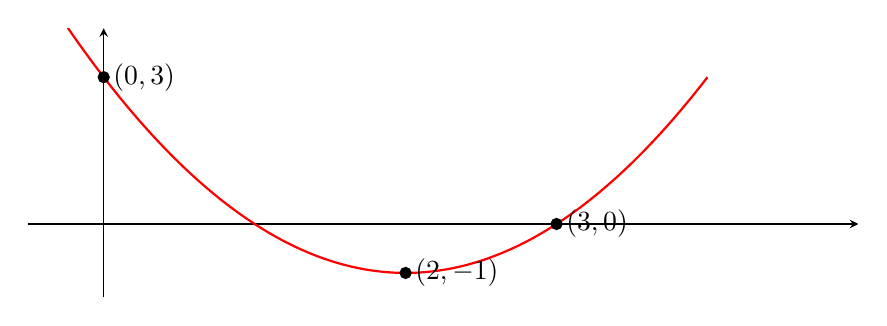
\begin{tikzpicture}
\begin{axis}[
    width=\linewidth,
    height=5cm,
    axis lines=middle,
    xmin=-0.5,xmax=5,
    ymin=-1.5,ymax=4,
    samples=100,
    ticks=none
]

% cubic
\addplot[red, thick, domain=-0.5:4] {x^2 - 4*x + 3};

% data points
\addplot[only marks,mark=*,mark size=2pt] 
coordinates {(0,3) (2,-1) (3,0)};
\node[right] at (0,3) {$(0,3)$};
\node[right] at (2,-1) {$(2,-1)$};
\node[right] at (3,0) {$(3,0)$};
\end{axis}
\end{tikzpicture}
\end{figure}
\begin{itemize}
    \item Solving the linear system gives $a_0=3$, $a_1=-4$, $a_2=1$ so the fit is 
    $$
    p(x)=  x^2 -4x  +3
    $$
\end{itemize}
    
\end{frame}

%%%%%%%%%%%%%%%%%%%%%%%%%%%%%%%%%%%%%%%%%%%%%%%%%%%%%%
\begin{frame}{General Interpolation with Monomials}
\begin{itemize}

\item Our polynomial of degree $n$ has $n+1$ unknown coefficients
  \begin{equation*}
    p_n(x) = a_0 + a_1 x + a_2 x^2 +\dots + a_{n} x^{n}
  \end{equation*}
\item There are $n+1$ conditions for the interpolation 
   $$p_n(x_i) = y_i, \quad \text{for} \; i=0,1,\ldots,n$$ 
\item Writing out all equations
  \begin{align*}
    a_0 + a_1 x_0 + a_2 x_0^2 +\dots + a_{n} x_0^{n} & = y_0\\
    a_0 + a_1 x_1 + a_2 x_1^2 +\dots + a_{n} x_1^{n} & = y_1\\
    a_0 + a_1 x_2 + a_2 x_2^2 +\dots + a_{n} x_2^{n} & = y_2\\
    a_0 + a_1 x_3 + a_2 x_3^2 +\dots + a_{n} x_3^{n} & = y_3\\
    \vdots &\\
    a_0 + a_1 x_n + a_2 x_n^2 +\dots + a_{n} x_n^{n} & = y_n\\
  \end{align*}
\end{itemize}
\end{frame}
%%%%%%%%%%%%%%%%%%%%%%%%%%%%%%%%%%%%%%%%%%%

\begin{frame}
\frametitle{The Vandermonde}
  \define{Vandermonde}{
    The matrix below is called the \textbf{Vandermonde matrix}, often labeled $V$.
  }
\begin{itemize}
    \item The system in matrix form: 
  \begin{align*}
    \begin{bmatrix}
      1 & x_0 & x_0^2 & \dots & x_0^{n}\\
      1 & x_1 & x_1^2 & \dots & x_1^{n}\\
      1 & x_2 & x_2^2 & \dots & x_2^{n}\\
        &     &       & \vdots&      \\
      1 & x_n & x_n^2 & \dots & x_n^{n}\\
    \end{bmatrix}
    \begin{bmatrix}
      a_0\\
      a_1\\
      a_2\\
      \vdots\\
      a_n\\
    \end{bmatrix}
     =
    \begin{bmatrix}
      y_0\\
      y_1\\
      y_2\\
      \vdots\\
      y_n\\
    \end{bmatrix}
  \end{align*}
  \item Solving this system gives the coefficients to 
    \begin{equation*}
    p_n(x) = a_0 + a_1 x + a_2 x^2 +\dots + a_{n} x^{n}
  \end{equation*}
\end{itemize}
\end{frame}
%%%%%%%%%%%%%%%%%%%%%%%%%%%%%%%%%%%%%%%%%%%
% \begin{frame}{Simple Vandermonde Example}
% \begin{example}
%     Find the interpolating polynomial containing the points $(2,3)$ and $(4,7)$.
% \end{example}
% \begin{itemize}
%     \item[1.] Since $n=2$, the polynomial is  order $n-1=1$: 
%     $p_1(x) = a_0 + a_1 x$
    
%     \item[2.] Set up the  Vandermonde linear system 
% $$
%     \begin{bmatrix}
%       1 & 2 \\
%       1 & 4 \\
%     \end{bmatrix}
%     \begin{bmatrix}
%       a_0\\
%       a_1\\
%     \end{bmatrix}
%      =
%     \begin{bmatrix}
%       3\\
%       7\\
%     \end{bmatrix}
% $$
%     \item[3.] Then solve the system 
%         \begin{align*}
%             a_0 &= -1\\
%             a_1 &= 2
%         \end{align*}
%     \item[4.] Finally, substitute the solution into the polynomial
%         $$p_1(x) = -1 + 2x$$
% \end{itemize}
% \end{frame}
%%%%%%%%%%%%%%%%%%%%%%%%%%%%%%%%%%%%%%%%%%%
\begin{frame}{Monomial Interpolation}

\method{Monomial Interpolation}{
$n+1$ data points $(x_i,y_i)$ 
}{
Degree $n$ polynomial cutting through all data points
}{
Set up an $(n+1)\times (n+1)$ matrix and solve it to find polynomial coefficients
}

\begin{itemize}
    \item If you use a \textbf{monomial basis}
    $$ \mathcal{F}= \{1, x, x^2, x^3,\ldots \}$$ 
    then your interpolation has the familiar form 
      \begin{equation*}
    p_n(x) = a_0 + a_1 x + a_2 x^2 +\dots + a_{n} x^{n}
  \end{equation*}
    \item The unknown coefficients $a_0$, $a_1$, $\ldots$, $a_n$ can be found by solving the \textbf{Vandermonde} system
\end{itemize}
\end{frame}
%%%%%%%%%%%%%%%%%%%%%%%%%%%%%%%%%%%%%%%%%%%
\begin{frame}{An issue}
 \question{
      Can you identify a possible issue for solving this system?
 }
  \begin{align*}
    \begin{bmatrix}
      1 & x_0 & x_0^2 & \dots & x_0^{n}\\
      1 & x_1 & x_1^2 & \dots & x_1^{n}\\
      1 & x_2 & x_2^2 & \dots & x_2^{n}\\
        &     &       & \vdots&      \\
      1 & x_n & x_n^2 & \dots & x_n^{n}\\
    \end{bmatrix}
    \begin{bmatrix}
      a_0\\
      a_1\\
      a_2\\
      \vdots\\
      a_n\\
    \end{bmatrix}
     =
    \begin{bmatrix}
      y_0\\
      y_1\\
      y_2\\
      \vdots\\
      y_n\\
    \end{bmatrix}
  \end{align*}
  \begin{itemize}
      \item Suppose the points $x_0,\; x_1, \ldots, x_n $ are between 0 and 1
      \item What happens if $n$ is large?
  \end{itemize}
\end{frame}
%%%%%%%%%%%%%%%%%%%%%%%%%%%%%%%%%%%%%%%%%%%
\begin{frame}{Bad Example}


\begin{block}{Problem}
    Consider fitting a polynomial through the data points ($\epsilon_1$,-0.0045), ($\epsilon_2$,0.0068), and ($\epsilon_3$,-0.0008).
\end{block}

\begin{figure}
    \centering
    \begin{tikzpicture}
\begin{axis}[
    width=\linewidth,
    height=4cm,
    axis lines=middle,
    xmin=-0.1,xmax=1.1,
    ymin=-0.05,ymax=0.1,
    samples=100,
    ticks=none
]

\addplot[red, thick, domain=-0.1:1] {((x-0.11)*(x-0.33)*(x-0.77)*(x-0.88)};

% data points
\addplot[only marks,mark=*,mark size=2pt] 
coordinates {(0.2,-0.0045) (0.5,0.0068) (0.8,-0.0008)};
\end{axis}
\end{tikzpicture}
\end{figure}

Vandermonde Matrix after underflow
    \[
\begin{bmatrix}
1 & \epsilon_1 & \epsilon_1^2 \\
1 & \epsilon_2 & \epsilon_2^2 \\
1 & \epsilon_3 & \epsilon_3^2 \\
\end{bmatrix} \quad \longrightarrow \quad 
\begin{bmatrix}
1 & \epsilon_1 & 0 \\
1 & \epsilon_2 & 0 \\
1 & \epsilon_3 & 0 \\
\end{bmatrix} 
\]
\end{frame}
%%%%%%%%%%%%%%%%%%%%%%%%%%%%%%%%%%%%%%%%%%%
\begin{frame}{Ill-Conditioning!}
    \begin{center}
    \pgfimage[height=5cm]{figs/polys}
    \end{center}
    \keyidea{
    \begin{itemize}
        \item cond($V$) typically grows with $n$
        \item If cond($V$) is high, the coefficient $a_0$,$\dots$,$a_n$ are computed with poor precision
    \end{itemize}
    }
\end{frame}
%%%%%%%%%%%%%%%%%%%%%%%%%%%%%%%%%%%%%%%%%%%
\begin{frame}{Another Downside}

\begin{block}{Problem}
    Consider fitting a polynomial through the data points $(0,3)$, $(1,4)$, $(2,-1)$ and $(3,0)$.
\end{block}

\begin{itemize}
    \item It is easy to set up the linear system 
\[
\begin{bmatrix}
1 & 0 & 0 &0 \\
1 & 1 & 1 & 1 \\
1 & 2 & 4 & 8 \\
1 & 3 & 9 & 27
\end{bmatrix}
\begin{bmatrix}
a_0 \\
a_1 \\
a_2 \\
a_3 \\
\end{bmatrix}
=
\begin{bmatrix}
3 \\
4 \\
-1 \\
0
\end{bmatrix}
\]
\item It is difficult to find the interpolation by hand
\end{itemize}
\end{frame}

%%%%%%%%%%%%%%%%%%%%%%%%%%%%%%%%%%%%%%%%%%%
\sectionframe{Lagrange Interpolation}
%%%%%%%%%%%%%%%%%%%%%%%%%%%%%%%%%%%%%%%%%%%

\begin{frame}{Another Basis}

\begin{block}{Monomial Basis}
    Monomials are the family of functions 
    $$ \mathcal{F}= \{1, x, x^2, x^3,\ldots \}$$
    \begin{itemize}
        \item Form a basis for polynomials 
        \item A natural choice  
        \item Suffers from some drawbacks for interpolation
    \end{itemize}
\end{block}

{
\question{Is there another basis for polynomials?}
}

\end{frame}


%%%%%%%%%%%%%%%%%%%%%%%%%%%%%%%%%%%%%%%%%%%
\begin{frame}{Consider this function $p(x)$}

\question{
Suppose you have two data points: $(x_0,y_0)$ and $(x_1,y_1)$. 
What is the behavior of the following function?
\begin{equation*} 
  p(x) = \left(\frac{x-x_1}{x_0-x_1}\right) y_0 + 
         \left(\frac{x-x_0}{x_1-x_0}\right) y_1
\end{equation*}
}

\begin{itemize}
  \item $p(x)$ is a degree 1 polynomial
  \item $\ell_0(x)$ is zero at $x_1$ and 1 at $x_0$
  \item $\ell_1(x)$ is zero at $x_0$ and 1 at $x_1$
  \item Thus $p(x_0)=y_0$ and $p(x_1) = y_1$
  \item These two are called \textbf{ Lagrange basis functions}:
    \begin{equation*}
      \ell_0(x) = \frac{x-x_1}{x_0-x_1}\qquad \ell_1(x) =\frac{x-x_0}{x_1-x_0}
    \end{equation*}
\end{itemize}
\end{frame}
%%%%%%%%%%%%%%%%%%%%%%%%%%%%%%%%%%%%%%%%%%%

%%%%%%%%%%%%%%%%%%%%%%%%%%%%%%%%%%%%%%%%%%%
\begin{frame}{Lagrange Basis Functions for Two Points}

\begin{columns}
\column{0.55\textwidth}

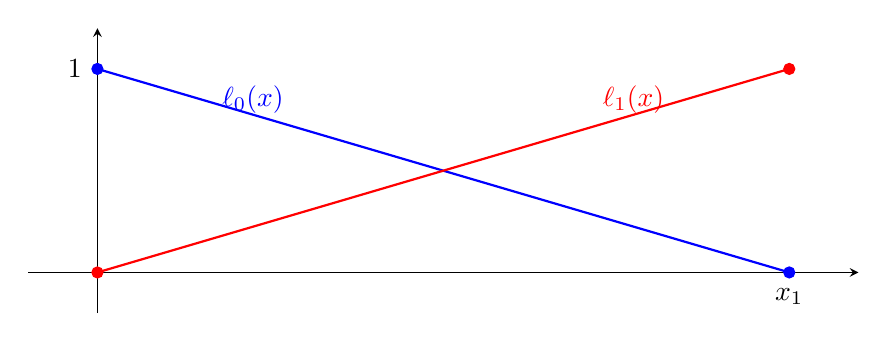
\begin{tikzpicture}
\begin{axis}[
    width=\linewidth,
    height=5.2cm,
    axis lines=middle,
    xmin=-0.2, xmax=2.2,
    ymin=-0.2, ymax=1.2,
    xtick={0,2},
    xticklabels={$x_0$,$x_1$},
    ytick={0,1},
    yticklabels={$0$,$1$},
    samples=100,
    domain=0:2,
    clip=false
]

% l0(x) = (x-x1)/(x0-x1) with x0=0, x1=2
\addplot[blue, thick] {(x-2)/(0-2)};
\addplot[blue, only marks, mark=*, mark size=2pt] coordinates {(0,1) (2,0)};
\node[blue] at (axis cs:0.45,0.85) {$\ell_0(x)$};

% l1(x) = (x-x0)/(x1-x0) with x0=0, x1=2
\addplot[red, thick] {(x-0)/(2-0)};
\addplot[red, only marks, mark=*, mark size=2pt] coordinates {(0,0) (2,1)};
\node[red] at (axis cs:1.55,0.85) {$\ell_1(x)$};

\end{axis}
\end{tikzpicture}

\column{0.45\textwidth}

\begin{block}{Key Properties}
\[
\ell_0(x_0)=1,\qquad \ell_0(x_1)=0
\]
\[
\ell_1(x_0)=0,\qquad \ell_1(x_1)=1
\]
\end{block}

\vspace{2mm}

\begin{itemize}
    \item Each basis function is 1 at its own node
    \item Each basis function is 0 at the other node
    \item Together they build the interpolating line
\end{itemize}

\[
p(x)=y_0\ell_0(x)+y_1\ell_1(x)
\]

\end{columns}

\end{frame}
%%%%%%%%%%%%%%%%%%%%%%%%%%%%%%%%%%%%%%%%%%%
\begin{frame}{Lagrange Basis Functions}
\define{Lagrange Basis Functions}{
    Let $x_0$, $x_1$, $\ldots$, $x_n$ be distinct points.
    \textbf{Lagrange basis functions} are a family of functions 
    $$\mathcal{F} = \{ \ell_0(x), \ell_1(x),\ldots, \ell_n(x) \}$$ satisfying  
    \begin{equation*}
  \ell_k(x) = \prod_{i=0,i\ne k}^{n} \frac{x-x_i}{x_k - x_i}, \text{ for } k=0,\ldots,n
\end{equation*}
    }
\bigskip
Properties:
\begin{itemize}
    \item  Each member $\ell_k(x)$ is a degree n polynomial
    \item When you evaluate $\ell_k$ at $x_k$, you get 1
    $\ell_i(x_i) = 1$
    \item $\ell_i(x_j) = 0$ whenever $i \neq j$
\end{itemize}
\end{frame}
%%%%%%%%%%%%%%%%%%%%%%%%%%%%%%%%%%%%%%%%%%%
% \begin{frame}{Lagrange Basis Functions for $n=2$}
% Suppose we have 3 points $(x_0, y_0)$, $(x_1,y_1)$, and $(x_2,y_2)$\\[5mm]
% Then our Lagrange basis functions are $\mathcal{F} = \{ \ell_0(x), \ell_1(x), \ell_2(x) \}$\\[5mm] 

% Properties: 
% \begin{itemize}
%     \item Each member $\ell_i(x)$ is a degree 2 polynomial
%     \item $\ell_i(x_i) = 1$
%     \item $\ell_i(x_j) = 0$ whenever $i \neq j$
% \end{itemize}

% \begin{example}
%     The Lagrange basis function $\ell_2(x)$ has the form 
%         $$\ell_2(x) = \frac{(x-x_0)(x-x_1)}{(x_2-x_0)(x_2-x_1)}$$
% \end{example}
% \end{frame}
%%%%%%%%%%%%%%%%%%%%%%%%%%%%%%%%%%%%%%%%%%%
\begin{frame}{Lagrange Basis for 3 Points}
\begin{example}
 Find the first Lagrange basis function $\ell_0(x)$ for the data points $(1,6), (-1,2),$ and $(2,12)$.
\end{example}
\begin{itemize}
    \item First, $\ell_0(x)$ must be zero $x_1=-1$ and $x_2=2$ so we write
    $$
    \ell_0(x) = (x+1)(x-2)
    $$
    \item Next, we find the correcting scalar. We want $\ell(x)=1$ at $x_0=1$

    \item Plug in $x_0$
    $$
    \ell_0(1)= (1+1)(1-2)= -2 
    $$
    \item We must \textit{correct} $\ell_0$ by scaling it by $-2$
    $$
        \ell_0(x) = -\frac{1}{2}(x+1)(x-2)
    $$
\end{itemize}
\end{frame}
%%%%%%%%%%%%%%%%%%%%%%%%%%%%%%%%%%%%%%%%%%%
\begin{frame}{Sanity Check}
\question{
Does the function     
    $$
        \ell_0(x) = -\frac{1}{2}(x+1)(x-2)
    $$
satisfy the properties of a Lagrange basis function for 
\begin{center}
  \begin{tabular}{c| c  c  c}
  $x$ & $1$ & $-1$ &$2$\\\hline
  $y$ & $6$ & $2$ &$12$\\
  \end{tabular} ?
\end{center}
}
\begin{itemize}
    \item $\ell_0(1)  =-\frac{1}{2}(1+1)(1-2)=1 \checkmark$
    \item $\ell_0(-1)  =-\frac{1}{2}(-1+1)(-1-2)=0 \checkmark$
    \item $\ell_0(2)  =-\frac{1}{2}(2+1)(2-2)=0 \checkmark$
\end{itemize}
{
\keyidea{
\begin{itemize}
    \item Lagrange basis functions act like a swicth: 0 or 1
    \item $\ell_0(x)$ is switched on at $x=x_0$
    \item $\ell_0(x)$ is switched off at $x=x_1$ and $x=x_2$
\end{itemize}
}
}
\end{frame}
%%%%%%%%%%%%%%%%%%%%%%%%%%%%%%%%%%%%%%%%%%%
\begin{frame}{Interpolation}

\begin{block}{Data}
    \begin{center}
  \begin{tabular}{c| c  c  c}
  $x$ & $1$ & $-1$ &$2$\\\hline
  $y$ & $6$ & $2$ &$12$\\
  \end{tabular} 
\end{center}
\end{block}
\begin{itemize}
    \item We found $\ell_0(x)$. We can find $\ell_1(x)$ and $\ell_2(x) $ similarly

    \item Then we can construct the interpolation  
    $$
    p(x)  = \ell_0(x) +2 \ell_1(x) + 12 \ell_2(x)
    $$
    \item At $x=x_0$
    $$
    p(x_0)  = \ell_0(x_0) +\cancel{2\ell_1(x_0)} + \cancel{12\ell_2(x_0)} = 1
    $$
    \item At $x=x_1$
    $$
    p(x_1)  = \cancel{\ell_0(x_1)} +2\ell_1(x_1) + \cancel{12\ell_2(x_1)} = 2
    $$
    \item At $x=x_2$
    $$
    p(x_1)  = \cancel{\ell_0(x_1)} +\cancel{2\ell_1(x_0)} + 12\ell_2(x_1) = 12
    $$
\end{itemize}
\end{frame}

%%%%%%%%%%%%%%%%%%%%%%%%%%%%%%%%%%%%%%%%%%%
\begin{frame}{Lagrange Interpolation Example}{Part 1}
\begin{example}
  Find the Lagrange interpolation for the data set $(1,6), (-1,2),$ and $(2,12)$.
\end{example}
\begin{itemize}
     \item Calculate $\ell_0$: $k=0$, $i=1,2$
\begin{align*}
  \ell_0(x) =\frac{(x-x_1)(x-x_2)}{(x_0-x_1)(x_0-x_2)} 
        = \frac{(x+1)(x-2)}{(2)(-1) } =-\frac{1}{2}(x+1)(x-2)
\end{align*}
\item Calculate $\ell_1$: $k=1$, $i=0,2$
\begin{align*}
  \ell_1(x)  = \frac{(x-x_0)(x-x_2)}{(x_1-x_0)(x_1-x_2)} 
        = \frac{(x-1)(x-2)}{(-2)(-3) } = \frac{1}{6}(x-1)(x-2)
\end{align*}
\item Calculate $\ell_2$: $k=2$, $i=0,1$
\begin{align*}
  \ell_2(x) = \frac{(x-x_0)(x-x_1)}{(x_2-x_0)(x_2-x_1)} 
        = \frac{(x-1)(x+1)}{(1)(3) } = \frac{1}{3}(x-1)(x+1)
\end{align*}
\end{itemize}
\end{frame}

%%%%%%%%%%%%%%%%%%%%%%%%%%%%%%%%%%%%%%%%%%%
\begin{frame}{Lagrange Interpolation Example}{Part 2}
\begin{example}
  Write the three Lagrange basis functions for the data points $(1,6), (-1,2),$ and $(2,12)$.
\end{example}

\begin{itemize}
    \item Then write the linear combination of the Lagrange basis functions 
    \begin{align*}
        p(x) &= y_0 \ell_0(x) + y_1 \ell_1(x) + y_2 \ell_2(x)\\
         &=  \ell_0(x) + 2\ell_1(x) + 12\ell_2(x)\\
         &=  -\frac{1}{2}(x+1)(x-2) + \frac{2}{6}(x-1)(x-2) + \frac{12}{3}(x-1)(x+1)\\
    \end{align*}

\end{itemize}

\end{frame}

%%%%%%%%%%%%%%%%%%%%%%%%%%%%%%%%%%%%%%%%%%%
\begin{frame}{Lagrange Interpolation}

\keyidea{

    \begin{itemize}
        \item Since Lagrange basis functions have a switch-like property,
             $$ y_k\; \ell_k(x)$$
        will be $y_k$ at $x=x_k$ and be zero at all other points

        \item We may easily create interpolation polynomials using Lagrange functions as the basis: 
        $$ p(x) = y_0 \ell_0(x) + y_1\ell_1(x)+ \cdots + y_n \ell_n(x)$$
    \end{itemize}
}

\method{Lagrange Interpolation}{Data $n+1$ points $(x_i,y_i)$ for $i=0,\ldots,n$}{Interpolating polynomial $p_n(x)$}{With Lagrange basis functions the interpolation can easily be found by hand. (Solving a linear system is not required.)}
\end{frame}


% %%%%%%%%%%%%%%%%%%%%%%%%%%%%%%%%%%%%%%%%%%%
\sectionframe{Final Remarks}
% %%%%%%%%%%%%%%%%%%%%%%%%%%%%%%%%%%%%%%%%%%%
\begin{frame}{Summary}

\begin{block}{Monomial Basis}
$$ \mathcal{F}= \{1, x, x^2, x^3,\ldots \}$$
\begin{itemize}
    \item Leads to a linear system (Vandermonde matrix)
    \item Can be expensive and numerically unstable
\end{itemize}
\end{block}

\begin{block}{Lagrange Basis}
$$\mathcal{F} = \{ \ell_0(x), \ell_1(x),\ldots, \ell_n(x) \}$$ 
\[
\ell_k(x) = \prod_{i=0,i\ne k}^{n} \frac{x-x_i}{x_k - x_i}
\]

\begin{itemize}
    \item Avoids solving a linear system
    \item Gives an explicit formula for $p(x)$
    \item But has limited flexibility
\end{itemize}
\end{block}

\end{frame}

%%%%%%%%%%%%%%%%%%%%%%%%%%%%%%%%%%%%%%%%%%%
\begin{frame}{Limitations of Lagrange Interpolation}

\begin{itemize}

\item \textbf{Adding a new data point is expensive}
\begin{itemize}
    \item If we add $(x_{n+1}, y_{n+1})$, we must recompute all basis functions
    \item The entire polynomial must be rebuilt from scratch
\end{itemize}

\vspace{3mm}

\item \textbf{No reuse of previous work}
\begin{itemize}
    \item We cannot easily update the polynomial incrementally
\end{itemize}

\vspace{3mm}

\item \textbf{Not ideal for computation}
\begin{itemize}
    \item Expression becomes complicated for large $n$
    \item Difficult to evaluate efficiently
\end{itemize}

\end{itemize}

\keyidea{
Lagrange interpolation is conceptually simple, but not computationally efficient.
}

\end{frame}

%%%%%%%%%%%%%%%%%%%%%%%%%%%%%%%%%%%%%%%%%%%
\begin{frame}[fragile]{Psuedocode}

% \begin{columns}
% \column{0.450\textwidth}
Just solve a linear system.
\begin{lstlisting}[language=matlab,caption=monomial]
Create vandermonde matrix V
Create b vector
Solve a=V\b
Construct polynomial
\end{lstlisting}

% \column{0.45\textwidth}
Create a domain vector, and construct $p(x)$ as a vector.
\begin{lstlisting}[language=matlab,caption=monomial]
xx = linspace(x0,xn)
p = zeros(size(xx))
for i=1:n
    Initialize li 
    for j = 0:n (skip i) 
        li = li + (xx-xi)./(xj-xi)
    end
end
\end{lstlisting}
% \end{columns}
\end{frame}
%%%%%%%%%%%%%%%%%%%%%%%%%%%%%%%%%%%%%%%%%%%
\begin{frame}{Moving Forward: Newton Interpolation}

\begin{block}{Idea}
Can we build the interpolating polynomial \textbf{incrementally}?
\end{block}

\begin{itemize}

\item Start with one data point $\{x_0\}$
\item Add one point at a time $\{x_0, x_1\}$
\item Update the polynomial without recomputing everything

\vspace{3mm}

\item This leads to a new representation:
\[
p(x) = c_0 
      + c_1(x-x_0)
      + c_2(x-x_0)(x-x_1)
      + \cdots
\]

\item Next lecture, we will introduce a third basis: \textbf{the Newton Polynomial basis functions} 
\end{itemize}


\end{frame}

% \begin{frame}{Lagrange Interpolation Example}
% \begin{example}
% Find the Lagrange interpolating polynomial passing through the points  $(1,6)$, $(-1,2)$, and $(2,12)$.\\
% \end{example}

% \begin{itemize}
%     \item[1.] From the previous example, we already found our basis functions:
% \[
% \begin{array}{llll} 
% \ell_0 (x) & = & \frac{(x-x_1)(x-x_2)}{(x_0-x_1)(x_0-x_2)} & 
%         = -\frac{1}{2}(x+1)(x-2)  \\
% \ell_1 (x) & = & \frac{1(x-x_0)(x-x_2)}{(x_1-x_0)(x_1-x_2)} & 
%         = \frac16{(x-1)(x-2)} \\
% \ell_2 (x) & = & \frac{(x-x_0)(x-x_1)}{(x_2-x_0)(x_2-x_1)} & 
%         = \frac13{(x-1)(x+1)} \\
% \end{array} 
% \] 
% \item[2.] Next, we write the general form for $n=3$ points
% $$
% p_2(x)  = y_0 \ell_0(x) + y_1 \ell_1(x) + y_2 \ell_2(x) 
% $$
% \item[3.] Finally, we substitute the values for $y_k$ and $\ell_k$
% \begin{eqnarray*} 
% p_2(x)   = -\frac{6}{2}(x+1)(x-2)  + \frac{2}{6}{(x-1)(x-2)}+ \frac{12}{3}{(x-1)(x+1)} \\ 
% \end{eqnarray*}
% \end{itemize}
% \end{frame}

% %%%%%%%%%%%%%%%%%%%%%%%%%%%%%%%%%%%%%%%%%%%
% \begin{frame}{Interpolation}
% \begin{center}
    
% \begin{tikzpicture}
%     \begin{axis}[
%         width=10cm, height=6cm,
%         xlabel={$x$}, ylabel={$y$},
%         grid=major, 
%         thick,
%         domain=-3:3,
%         samples=100,
%         % legend pos=outer south
%     ]
%     % Polynomial interpolation curve
%     \addplot[color=blue, thick] {-3*(x+1)*(x-2) + 0.333*(x-1)*(x-2) + 4*(x-1)*(x+1)};

%     % Interpolation points
%     \addplot[color=red, only marks, mark=*] 
%         coordinates {(-1,2) (1, 6) (2, 12)};
    
%     % Optional legend
%     \legend{Interpolation $g(x)$, Data Points};
%     \end{axis}
% \end{tikzpicture}\\
% \begin{itemize}
%     \item Data points: (-1,2), (1,6), (2,12) 
%     \item Interpolation: $g(x) =  -3(x+1)(x-2) + \dfrac13 (x-1)(x-2) + 4(x-1)(x+1)$
% \end{itemize}
% \end{center}
% \end{frame}



\end{document}
